%%% Folie
\begin{frame}{Ausgangslage}
    Hier die Ausgangslage/Motivation für das Kapitel beschreiben ...

    % UNGEFÄHRE AUSSAGE
    %
    % Die einfachen Programmbeispiele der vorangegangen Kapitel eignen sich in der
    % Regel kaum für produktive Anwendungen, da sie einem einfachen, prozeduralen
    % Programmierstil gehorchen, bei dem jeder Methodenaufruf den rufenden Thread
    % so lange blockiert, bis die gewünschte Aktion durchgeführt wurde. Auf diese
    % Weise lassen sich daher nur sehr wenige Sensoren und Aktoren verbinden und
    % bestimmte Anwendungsfälle, wie die Bereitstellung einer deviceseitigen REST-API
    % lassen sich auf diese Weise gar nicht realisieren. Darüber hinaus wird der
    % Quellcode auch schnell sehr komplex und unübersichtlich, je mehr Komponenten
    % integriert werden sollen. Dieses Kapitel soll daher die wesentlichen
    % Architekturmuster zeigen, mit denen sich komplexe Pythonprogramme in lose
    % gekoppelte Einheiten zerlegen lassen, die eine einfache Erweiterbarkeit und
    % Wartbarkeit des Quellcodes (z.B. wenn eine Komponente ausgetauscht werden
    % muss) ermöglichen.
\end{frame}

%%% Folie
\begin{frame}{Lernziele}
    \begin{itemize}
        \item Komplexe Anwendungsfälle objektorientiert modellieren können
        \item Python-Anwendungen mit Klassen und Modulen modularisieren können
        \item Die Nachteile einer zu engen Kopplung von Klassen verstehen können
        \item Entwurfsmuster Observer und Message Broker anwenden können
        \item Nebenläufige Programmierung mit Threads in Python
        %\item Nebenläufige Programmierung mit Coroutinen in Python
    \end{itemize}
\end{frame}


%-------------------------------------------------------------------------------
\section{Design Patterns}
%-------------------------------------------------------------------------------

%%% Folie
\begin{frame}{Übersicht}
    TODO
\end{frame}

%%% Folie
\begin{frame}{DI und IOC Intro}
  Definition, GoF, Loose Coupling (Grafik)
\end{frame}

%%% Folie
\begin{frame}{DI und IOC Anwendungsfall}
   TODO
 \end{frame}
 
 %%% Folie
\begin{frame}{DI in Python Einfach}
TODO
  \end{frame}

%%% Folie
\begin{frame}{Container Injection}
TODO
  \end{frame}

%%% Folie
\begin{frame}{Python Konstrukte}
    Monkey Patching, Mixins
\end{frame}

%%% Folie
\begin{frame}{Testing mit MagicMock}
    TODO
\end{frame}

%%% Folie
\begin{frame}{Observer Pattern}
    Definition,Grafik
\end{frame}

%%% Folie
\begin{frame}{Publish-Subscribe}
   % https://hackernoon.com/observer-vs-pub-sub-pattern-50d3b27f838c
\end{frame}

%%% Folie
\begin{frame}{Anwendungsfall Teil 1 - Projektstruktur}
    TODO
\end{frame}

%%% Folie
\begin{frame}{Anwendungsfall Teil 2 - Code}
    TODO
\end{frame}

%%% Folie
\begin{frame}{Folie}
    TODO
\end{frame}

%%% Folie
\begin{frame}{Folie}
    TODO
\end{frame}

%%% Folie
\begin{frame}{Folie}
    TODO
\end{frame}

%%% Folie
\begin{frame}{Folie}
    TODO
\end{frame}

%-------------------------------------------------------------------------------
\section{Nebenläufigkeit in Python}
%-------------------------------------------------------------------------------

%%% Folie
\begin{frame}{Nebenläufigkeit vs. Parallelität - Intro}
        \begin{itemize}
        \setlength{\itemindent}{2.0in}
        \item [\textbf{Definition: Nebenläufig vs. Parallel}]
    \end{itemize}

    \begin{itemize}
        \item Als \textbf{nebenläufig} definieren wir Aufgaben, die auf einem Computer um Ressourcen konkurrieren und nicht notwendigerweise gleichzeitig ausgeführt werden (können)
        \item Als \textbf{parallel} definieren wir nebenläufige Aufgaben, die gleichzeitig ausgeführt werden (können)
     \end{itemize}
\end{frame}

\begin{frame}{Nebenläufigkeit vs. Parallelität -Beispiele}
        \begin{itemize}
        \setlength{\itemindent}{2.0in}
        \item [\textbf{Beispiele: Nebenläufig oder Parallel ?}]
    \end{itemize}

    \begin{itemize}
        \item Abfrage der Werte verschiedener angeschlossener Sensoren $\Rightarrow$ nebenläufig
        \item Schnelle unabhängige Sortierung von Werten $\Rightarrow$ (embarassingly) parallel
        \item Gleichzeitige Anzeige von Dashboard Daten und Erfassung der Messwerte $\Rightarrow$ nebenläufig
        \item Mathematische Transformationen (Filter, Computer Vision) auf Kamerabildern  $\Rightarrow$ parallel %http://files.hanser.de/Files/Article/ARTK_LPR_9783446449336_0001.pdf
        \item Versand von Nachrichten über das Internet aus verschiedenen Modulen eines Programms  $\Rightarrow$ nebenläufig
     \end{itemize}
\end{frame}

\begin{frame}{Raspberry PI 3 und Nebenläufigkeit}
     \begin{itemize}
        \setlength{\itemindent}{1.0in}
        \item [\textbf{Raspberry PI 3b}]
    \end{itemize}
    \begin{itemize}
        \item Quadcore CPU
        \item Benchmarks für z.B. Primzahlberechnung oder Unzip  mit deutlichem Geschwindigkeitsvorteil
     \end{itemize}
  \begin{figure}[!htb]
  \hspace*{-4cm}   
        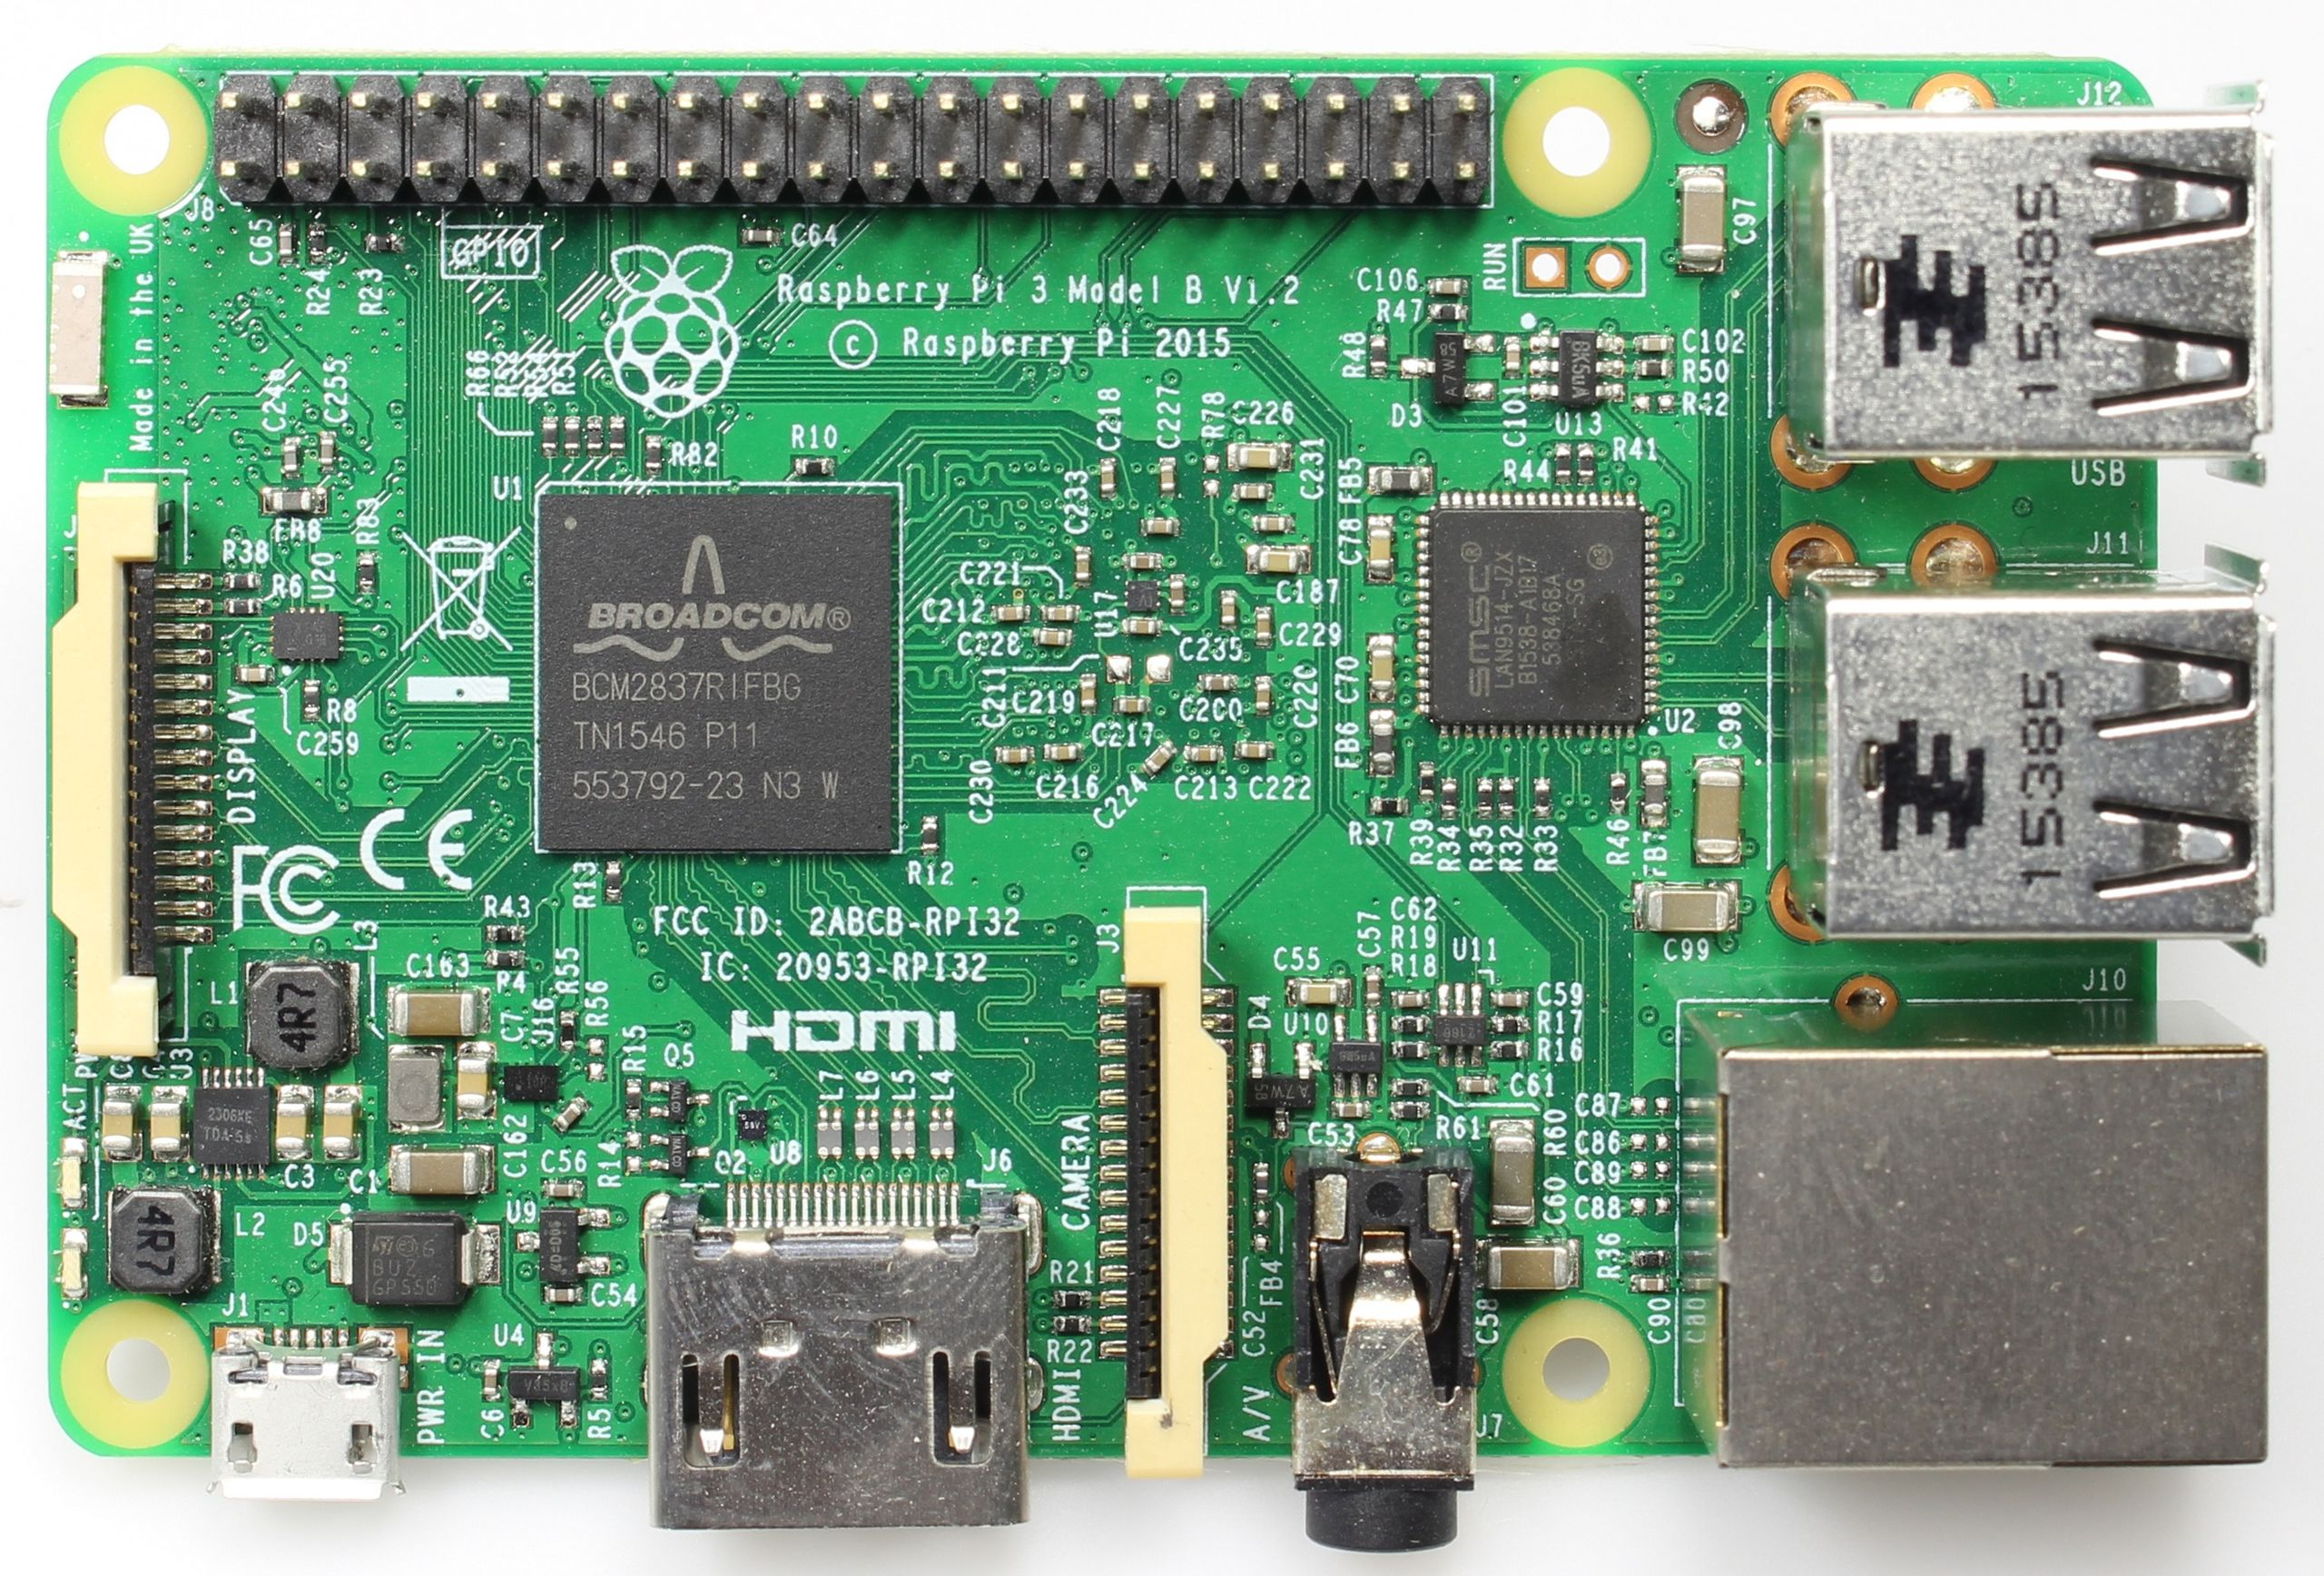
\includegraphics[scale=0.075]{6-python3/img/raspi3}  %https://upload.wikimedia.org/wikipedia/commons/thumb/4/49/Rasperry_pi_3_model_b_v1.3_bot.jpg/2560px-Rasperry_pi_3_model_b_v1.3_bot.jpg
    \end{figure}

\end{frame}

\begin{frame}{Raspberry PI 3 Cluster}
	  \begin{figure}[!htb]
        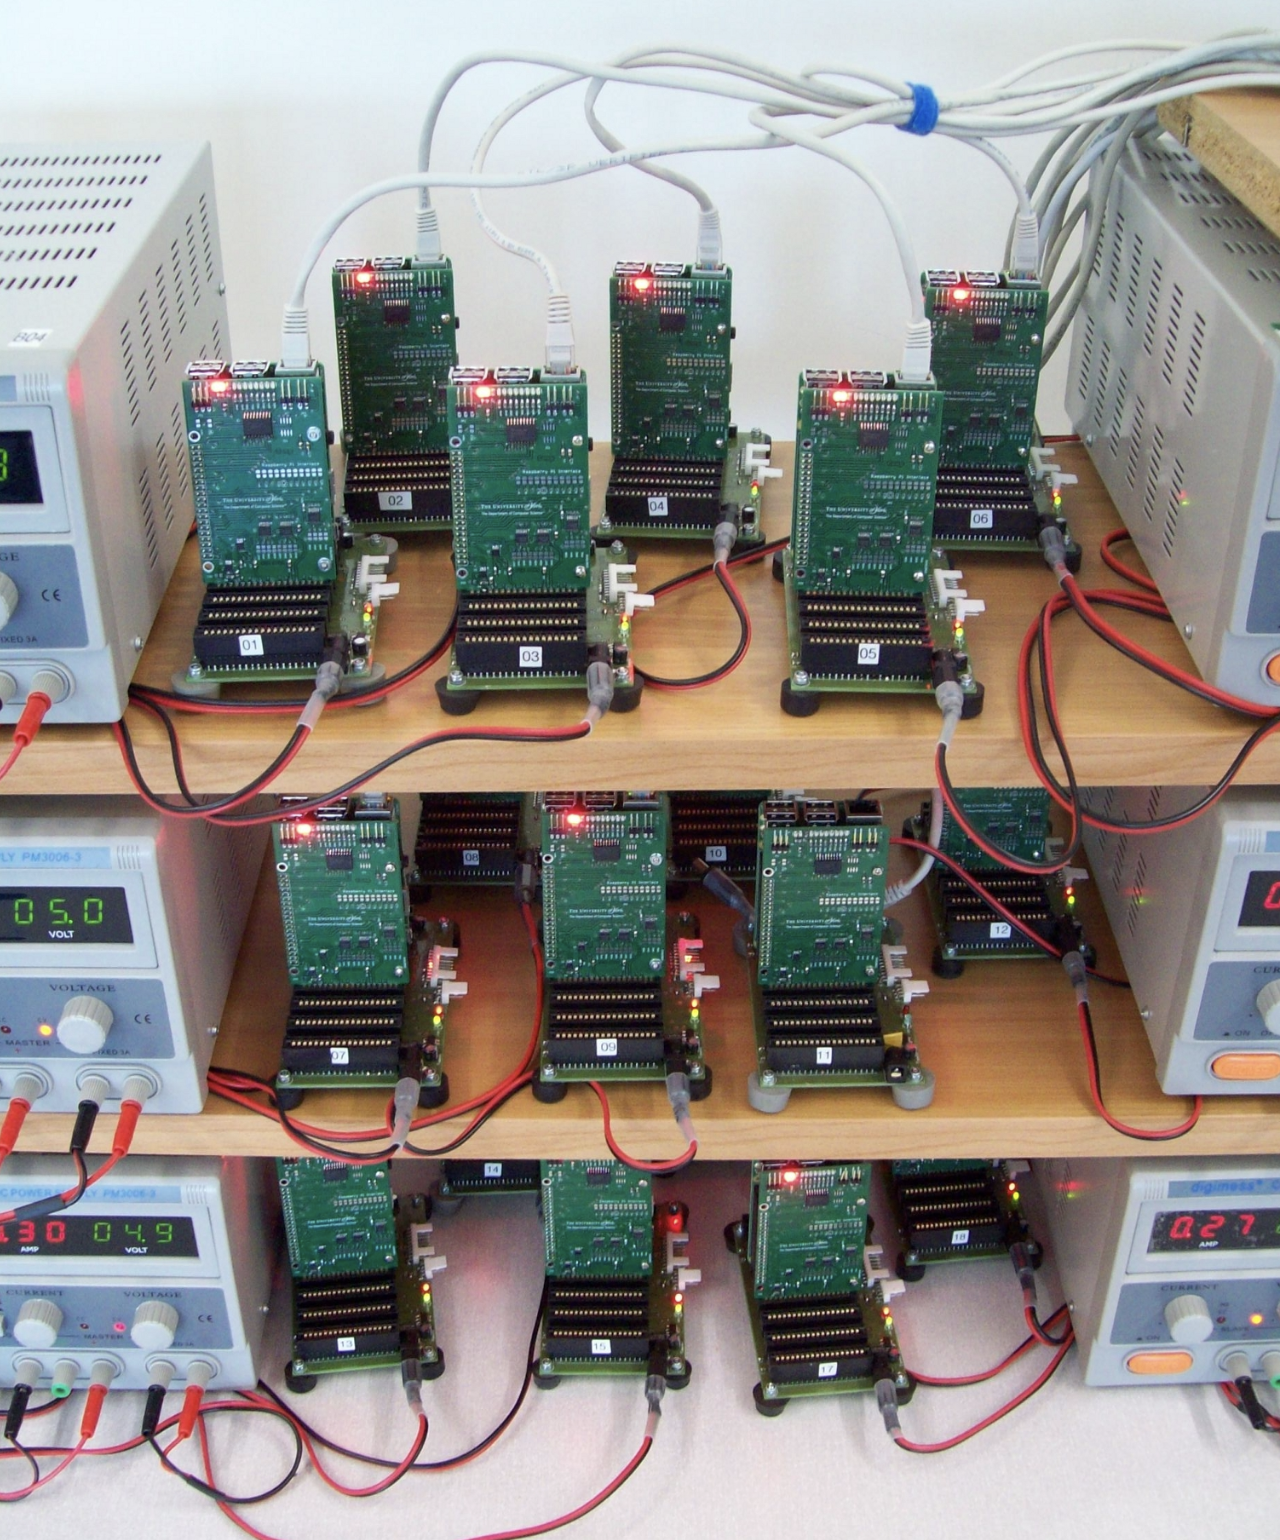
\includegraphics[scale=0.23]{6-python3/img/raspi3cluster}  %https://www-users.cs.york.ac.uk/~mjf/pi_cluster/Images/cluster1.jpg
    \end{figure}

\end{frame}

\begin{frame}{Recap: Threads vs. Prozesse}
    Definition, Zweck
\end{frame}



\begin{frame}{Python GIL}
    Definition, Zweck, Konsequenzen, andere Interpreter ohne GIL
\end{frame}

\begin{frame}{Python Multiprocessing Lib (kurz)}
    Module multiprocessing Übersicht
\end{frame}

%%% Folie
\begin{frame}{Threads in Python}
    Module thread (Hinweis Python2 vs Python 3), threading (detailliert)
\end{frame}

%%% Folie
\begin{frame}{Beispiel Ping mit Threads}
  %https://www.python-kurs.eu/threads.php
    \begin{figure}[!htb]
        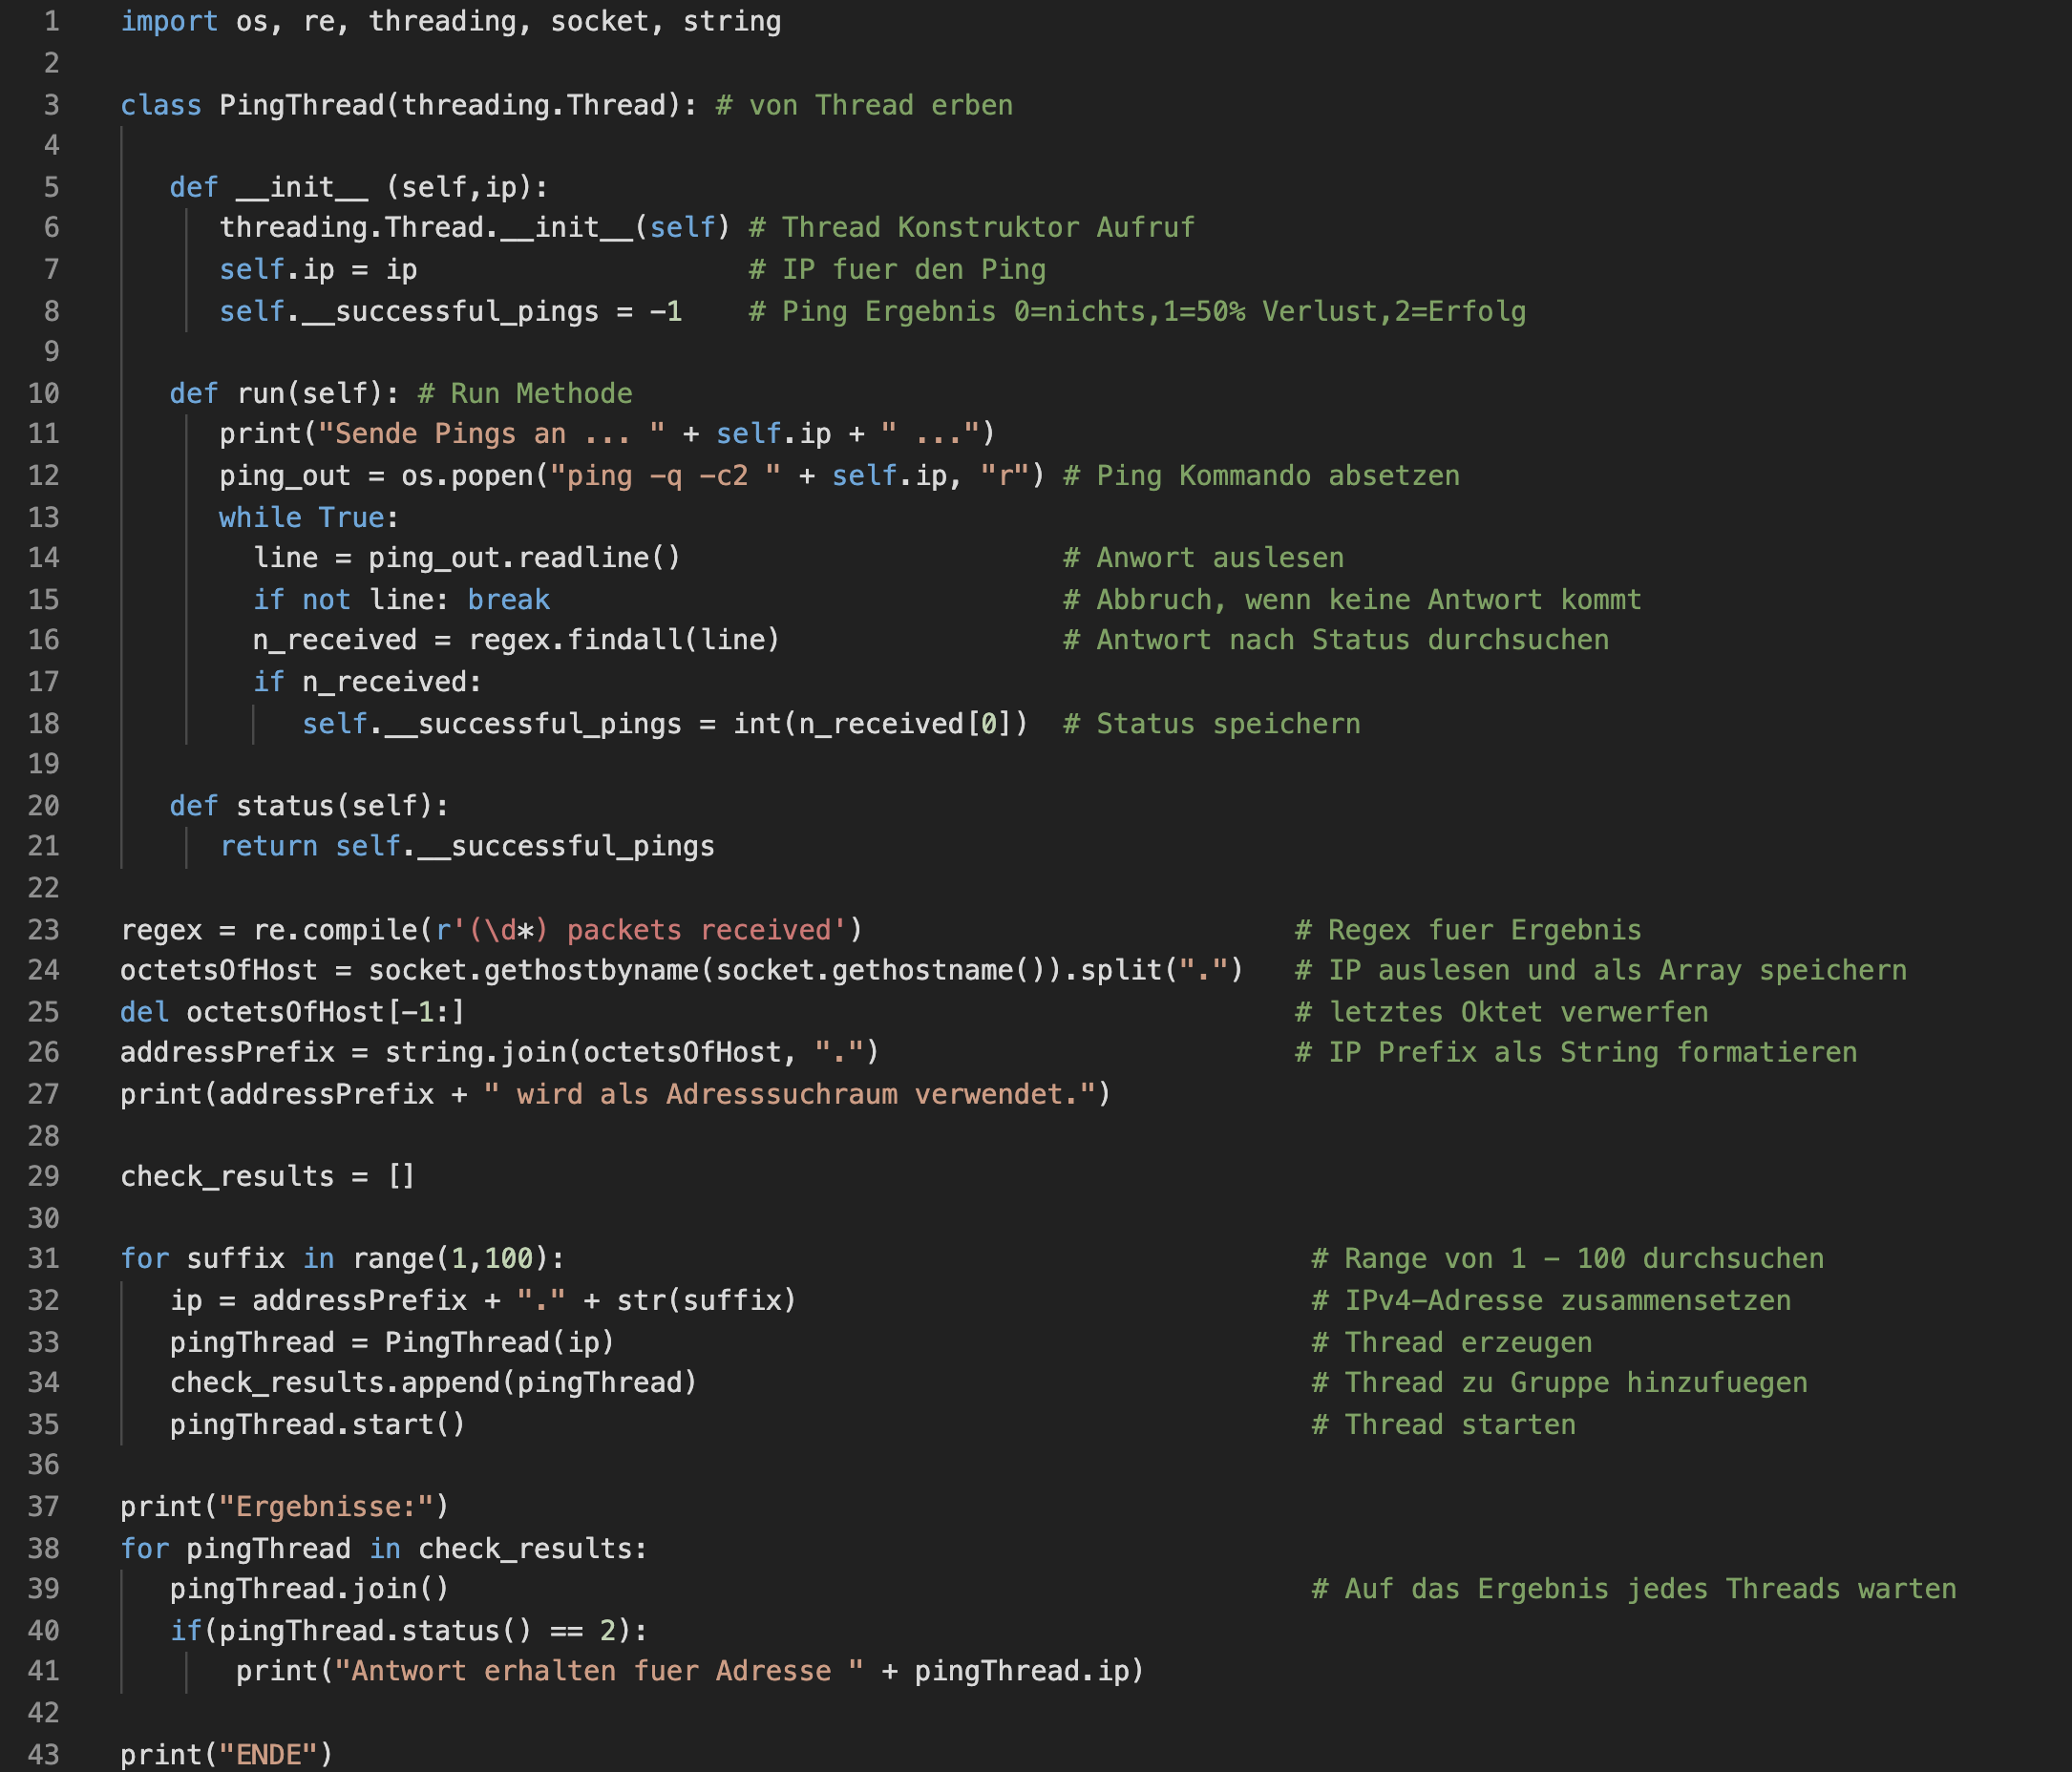
\includegraphics[scale=0.23]{6-python3/img/pingthreads}
    \end{figure}

\end{frame}

%%% Folie
\begin{frame}{Thread Probleme}
    Deadlock, Threads nicht starten wenn module Importiert wird etc.
\end{frame}

%%% Folie
\begin{frame}{Locks}
   Definition, Nutzen, with statement
\end{frame}


%%% Folie
\begin{frame}{Folie}
    TODO
\end{frame}

%%% Folie
\begin{frame}{Folie}
    TODO
\end{frame}

%%% Folie
\begin{frame}{Folie}
    TODO
\end{frame}

%%% Folie
\begin{frame}{Folie}
    TODO
\end{frame}

%%% Folie
\begin{frame}{Folie}
    TODO
\end{frame}

%%% Folie
\begin{frame}{Folie}
    TODO
\end{frame}

%%% Folie
\begin{frame}{Folie}
    TODO
\end{frame}

%%% Folie
\begin{frame}{Folie}
    TODO
\end{frame}

%%% Folie
\begin{frame}{Folie}
    TODO
\end{frame}

%%% Folie
\begin{frame}{Folie}
    TODO
\end{frame}

%%% Folie
\begin{frame}{Folie}
    TODO
\end{frame}


